\chapter{評価実験}\label{cha:Evaluation}

本研究で提案するプロンプトの有用性を検証するため、実験を行った。本実験の被験者は、システム仕様書作成経験のない学生4人である。
実験では、実際のシステム開発を想定した題材を用い、提案プロンプトを用いた手法とその他の手法で、被験者が章立てを作成する。作成した章立ての品質を、
株式会社スカイコム\cite{skycom}にて5年以上のシステム仕様書作成経験を持つ専門家5人が評価者となり、評価した。


\section{実験設定}

\subsection{対象システム}
\label{sec:target_system}

実験の題材として、以下の2つのシステムを選定した。
\begin{enumerate}
    \item \textbf{BMP画像分割アプリ}: BMP画像を指定された数に分割し、保存するアプリケーション
    \item \textbf{クラウド型電子契約サービス}: PDF技術を活かした電子契約/ワークフロー、それらに付随する文書管理、およびユーザー管理機能を持つクラウドサービス
\end{enumerate}

BMP画像分割アプリは機能が少ない単純なシステムとして、クラウド型電子契約サービスは機能が多い複雑なシステムとして、実験対象とした。

\subsection{比較手法}

システム仕様書章立ての作成手法として、以下の3パターンを設定した。
\begin{itemize}
    \item \textbf{手法A(手動作成)}: 被験者はLLMを用いず、章立てを作成する。この際、被験者には、対象システムの情報(\ref{sec:target_system}節を参照)と、ベースの章立て(図\ref{fig:base_outline}を参照)を与える。
    \item \textbf{手法B(自由プロンプト)}: 被験者はLLM(GPT-5.2)を使用して、章立てを作成する。この際、被験者には、対象とするシステムの情報(\ref{sec:target_system}節を参照)と、ベースの章立て(図\ref{fig:base_outline}を参照)を与える。ただし、提案プロンプトは与えずに、被験者自身による自由なプロンプトをLLM(GPT-5.2)に与える。
    \item \textbf{手法C(提案プロンプト)}: 被験者はLLM(GPT-5.2)を使用し、提案プロンプトを用いて章立てを作成する。
\end{itemize}

図\ref{fig:bmp}にBMP画像分割アプリを対象とした手法Cで用いるプロンプトの「開発するシステム情報」部分を示す。
\begin{figure}[tp]
\begin{tcolorbox}[
  colback=white,
  colframe=blue,
  fonttitle=\bfseries,
]
\footnotesize
\ttfamily
\fontsize{10}{11}\selectfont
\begin{verbatim}
【開発するシステム情報】
- システム名：BMP画像分割アプリ
- 概要：指定されたBMP画像ファイルを指定された数に分割する。
\end{verbatim}
\end{tcolorbox}
% \par\vspace{-20pt}
\captionof{figure}{BMP画像分割アプリを対象とした手法Cで用いるプロンプトの「開発するシステム情報」部分}
\label{fig:bmp}
\end{figure}

図\ref{fig:cloud}にクラウド型電子契約サービスを対象とした手法Cで用いるプロンプトの「開発するシステム情報」部分を示す。
\begin{figure}[tp]
\begin{tcolorbox}[
  colback=white,
  colframe=blue,
  fonttitle=\bfseries,
]
\footnotesize
\ttfamily
\fontsize{10}{11}\selectfont
\begin{verbatim}
【開発するシステム情報】
- システム名：クラウド型電子契約サービス
- 概要：PDF技術を活かした電子契約/ワークフロー、それらに付随する文書管理、およびユーザー管理機能を持つクラウドサービス
\end{verbatim}
\end{tcolorbox}
% \par\vspace{-20pt}
\captionof{figure}{クラウド型電子契約サービスを対象とした手法Cで用いるプロンプトの「開発するシステム情報」部分}
\label{fig:cloud}
\end{figure}

\subsection{被験者と実験の割り当て}

表\ref{tb:experiment_allocation}に、被験者ごとの対象システムと手法の割り当てを示す。

\begin{table}[tp]
  \caption{被験者ごとの対象システムと手法の割り当て}
  \label{tb:experiment_allocation}
  \centering
  \begin{tabular}{|c|l|l|}
    \hline
    \textbf{被験者} & \textbf{BMP画像分割アプリ} & \textbf{クラウド型電子契約サービス} \\
    \hline\hline
    A & 手法A(手動) & 手法C(提案プロンプト) \\
    \hline
    B & 手法C(提案プロンプト) & 手法A(手動) \\
    \hline
    C & 手法B(自由プロンプト) & 手法C(提案プロンプト) \\
    \hline
    D & 手法C(提案プロンプト) & 手法B(自由プロンプト) \\
    \hline
  \end{tabular}
\end{table}

\subsection{評価方法}
作成した章立ては、株式会社スカイコムにて5年以上のシステム仕様書作成経験を持つ専門家が評価者となり、評価した。
評価は以下の9項目について行い、それぞれ5段階のリッカート尺度\cite{likert}(5:非常に良い, 4:良い, 3:普通, 2:悪い, 1:非常に悪い)で採点した。

\begin{enumerate}
  \item 最低限含むべき章を含んでいるか(網羅性)
  \item 章の順序は適切か(論理性)
  \item 章タイトルは適切か(命名の適切さ)
  \item 章立て全体として理解しやすいか(可読性)
  \item 章の粒度は適切か(粒度の適切さ)
  \item 想定読者に適した章立てか(適合性)
  \item 将来的な拡張に対応しやすい章立てか(拡張性)
  \item 章、節、項の包含関係は適切か(構造的整合性)
  \item 章立てがシステム独自の章立てになっているか(独自性)
\end{enumerate}

また、これら9項目の定量的な評価に加え、各対象システムに対して、評価者から全体的な所感や各手法に対する改善点を自由記述形式のコメントとして収集した。
そのため、すべての章立てに対して個別のコメントが得られているわけではないが、得られたコメントについては\ref{sec:evaluation_results}節で示す。



% \begin{enumerate}
%     \item 最低限含むべき章を含んでいるか(網羅性)
%     \begin{itemize}
%         \item 5: すべて含まれている
%         \item 4: 軽微な不足がある
%         \item 3: 一部重要な章が不足している
%         \item 2: 多くの重要な章が不足している
%         \item 1: 最低限必要な章が1つも含まれていない
%     \end{itemize}
%     \item 章の順序は適切か(論理性)
%     \begin{itemize}
%         \item 5: 非常に適切
%         \item 4: 概ね適切
%         \item 3: 一部不適切
%         \item 2: 不適切な章順序が多い
%         \item 1: 全体的に不適切
%     \end{itemize}
%     \item 章タイトルは適切か(命名の適切さ)
%     \begin{itemize}
%         \item 5: 非常に適切
%         \item 4: 概ね適切
%         \item 3: 一部不適切
%         \item 2: 不適切な章タイトルが多い
%         \item 1: 全体的に不適切
%     \end{itemize}
%     \item 章立て全体として理解しやすいか(可読性)
%     \begin{itemize}
%         \item 5: 非常に理解しやすい
%         \item 4: 理解しやすい
%         \item 3: 普通
%         \item 2: 理解しにくい
%         \item 1: 非常に理解しにくい
%     \end{itemize}
%     \item 章の粒度は適切か(粒度の適切さ)
%     \begin{itemize}
%         \item 5: 非常に適切
%         \item 4: 概ね適切
%         \item 3: 普通
%         \item 2: 過不足が多い
%         \item 1: 非常に過不足が多い
%     \end{itemize}
%     \item 想定読者に適した章立てか(適合性)
%     \begin{itemize}
%         \item 5: 非常に適切
%         \item 4: 概ね適切
%         \item 3: 一部不適切
%         \item 2: 不適切な章が多い
%         \item 1: 全体的に不適切
%     \end{itemize}
%     \item 将来的な拡張に対応しやすい章立てか(拡張性)
%     \begin{itemize}
%         \item 5: 非常に拡張しやすい
%         \item 4: 拡張しやすい
%         \item 3: 普通
%         \item 2: 拡張しにくい
%         \item 1: 非常に拡張しにくい
%     \end{itemize}
%     \item 章、節、項の包含関係は適切か(構造的整合性)
%     \begin{itemize}
%         \item 5: 非常に適切
%         \item 4: 概ね適切
%         \item 3: 一部不適切
%         \item 2: 不適切な包含関係が多い
%         \item 1: 全体的に不適切
%     \end{itemize}
%     \item 章立てがシステム独自の章立てになっているか(独自性)
%     \begin{itemize}
%         \item 5: システム固有の機能や特性が章立てに十分に反映されており、独自性が高い
%         \item 4: システム固有の要素が概ね反映されている
%         \item 3: 一部システム固有の要素があるが、汎用的な構成に近い
%         \item 2: 汎用的なテンプレートに近く、システム固有の要素が少ない
%         \item 1: 完全に汎用的なテンプレートであり、システム固有の要素がない
%     \end{itemize}
% \end{enumerate}

\section{評価結果}
\label{sec:evaluation_results}

\subsection{BMP画像分割アプリ}
本節では、実験において被験者が作成したBMP画像分割アプリの章立ての評価結果について述べる。

\subsubsection{手法A(手動作成)}
%評価結果の表(行が評価項目、列が評価者)
%章立て
%傾向の分析

図\ref{fig:A_chapter_structure_of_bmp_app}に、手法Aを用いて作成したBMP画像分割アプリの章立てを示す。
また、以下に評価者のコメントを示す。

\noindent\textbf{評価者のコメント}\\
評価者A：微妙\\
評価者C：書くべきことが書けていない\\
評価者E：シンプル\\


\begin{figure}[tp]
\begin{tcolorbox}[
  colback=white,
  colframe=orange,
  fonttitle=\bfseries
]
\begin{multicols}{2}
\footnotesize
\ttfamily
\fontsize{8}{9}\selectfont
\begin{verbatim}
1. 概要
 1.1.目的
 1.2.アプリケーションの概要
2. アプリケーションの基本条件
 2.1.入力画像の条件
 2.2.動作環境
 2.3.性能条件
3. 構成
 1.アプリケーションの構成
 2.ネットワークの構成
4. アプリケーションの機能
 4.1.単一画像分割機能
 4.2.複数枚分割機能
5. アプリケーションの運用
 5.1.運用方法
 5.2.障害時の運用
6.セキュリティ
7.安全設計
8.データ仕様
 8.1.コード体系
 8.2.データベース
 8.3.ファイル
 8.4.入出力データ
 8.5.メッセージ
9.付帯事項
\end{verbatim}
\end{multicols}
\end{tcolorbox}
\caption{手法AによるBMP画像分割アプリの章立て}
\label{fig:A_chapter_structure_of_bmp_app}
\end{figure}

表\ref{tb:detailed_evaluation_results_A}に、手法Aを用いて作成したBMP画像分割アプリシステム仕様書の章立ての評価結果を示す。

\begin{table}[tp]
  \caption{BMP画像分割アプリにおける手法A(手動作成)の評価者別詳細評価結果}
  \label{tb:detailed_evaluation_results_A}
  \centering
  \begin{tabular}{|l|c|c|c|c|c|c|}
    \hline
    \textbf{評価項目} & \textbf{評価者1} & \textbf{評価者2} & \textbf{評価者3} & \textbf{評価者4} & \textbf{評価者5} & \textbf{平均} \\
    \hline\hline
    1. 網羅性 & 2 & 5 & 3 & 3 & 5 & 3.6 \\
    \hline
    2. 論理性 & 3 & 4 & 4 & 4 & 5 & 4.0 \\
    \hline
    3. 命名の適切さ & 3 & 4 & 3 & 4 & 4 & 3.6 \\
    \hline
    4. 可読性 & 4 & 3 & 3 & 3 & 4 & 3.4 \\
    \hline
    5. 粒度の適切さ & 2 & 5 & 2 & 4 & 4 & 3.4 \\
    \hline
    6. 適合性 & 3 & 4 & 3 & 3 & 4 & 3.4 \\
    \hline
    7. 拡張性 & 4 & 4 & 3 & 4 & 4 & 3.8 \\
    \hline
    8. 構造的整合性 & 4 & 4 & 4 & 4 & 4 & 4.0 \\
    \hline
    9. 独自性 & 2 & 4 & 4 & 2 & 4 & 3.2 \\
    \hline
  \end{tabular}
\end{table}



\subsubsection{手法B(自由プロンプト)}
%評価結果の表(行が評価項目、列が評価者)
%章立て
%傾向の分析


図\ref{fig:B_chapter_structure_of_bmp_app}に、手法Bを用いて作成したBMP画像分割アプリの章立てを示す。
また、以下に評価者のコメントを示す。

\begin{figure}[tp]
\begin{tcolorbox}[
  colback=white,
  colframe=orange,
  fonttitle=\bfseries
]
\begin{multicols}{2}
\footnotesize
\ttfamily
\fontsize{8}{9}\selectfont
\begin{verbatim}
1. 概要
 1.1 目的
 1.2 システム概要
 1.3 用語・略語定義
2. システム基本条件
 2.1 動作環境
  2.1.1 対応OS
  2.1.2 実行形態
 2.2 対応BMPファイル仕様
  2.2.1 対応ビット深度
  2.2.2 非対応形式の扱い
 2.3 性能条件
  2.3.1 最大画像サイズ
  2.3.2 処理時間目安
 2.4 制約条件
  2.4.1 分割数の制約
  2.4.2 メモリ使用制約
3. システム構成
 3.1 全体構成
  3.1.1 処理フロー
  3.1.2 入出力関係
 3.2 ソフトウェア構成
  3.2.1 使用プログラミング言語
  3.2.2 使用ライブラリ
4. 機能仕様
 4.1 機能一覧
 4.2 画像入力機能
  4.2.1 入力方法
  4.2.2 入力チェック
 4.3 分割数指定機能
  4.3.1 指定方法
  4.3.2 不正値の扱い
 4.4 画像分割処理機能
  4.4.1 分割処理開始条件
  4.4.2 分割処理結果
 4.5 分割画像出力機能
  4.5.1 出力形式
  4.5.2 ファイル命名規則
5. 画像分割処理仕様
 5.1 分割方式
  5.1.1 縦横分割の定義
  5.1.2 均等分割の考え方
 5.2 端数処理
  5.2.1 幅方向の端数処理
  5.2.2 高さ方向の端数処理
 5.3 処理アルゴリズム概要
  5.3.1 ピクセル取得処理
  5.3.2 画像生成処理
6. 入出力仕様
 6.1 入力データ仕様
  6.1.1 入力ファイル
  6.1.2 入力パラメータ
 6.2 出力データ仕様
  6.2.1 出力ファイル構成
  6.2.2 出力先ディレクトリ
7. エラー処理・例外処理
 7.1 入力エラー
  7.1.1 ファイル未存在
  7.1.2 形式不正
 7.2 処理エラー
  7.2.1 メモリ不足
  7.2.2 分割処理失敗
8. 操作・運用
 8.1 操作手順
  8.1.1 起動
  8.1.2 処理実行
  8.1.3 終了
 8.2 エラー発生時の対応
  8.2.1 エラーメッセージ表示
  8.2.2 ユーザー対応
9. セキュリティ・安全設計
 9.1 ファイル操作上の安全性
 9.2 不正入力対策
10. 付帯事項
 10.1 既知の制限事項
 10.2 今後の拡張予定
\end{verbatim}
\end{multicols}
\end{tcolorbox}
\caption{手法BによるBMP画像分割アプリの章立て}
\label{fig:B_chapter_structure_of_bmp_app}
\end{figure}

\noindent\textbf{評価者のコメント}\\
評価者A：冗長\\
評価者B：冗長\\
評価者C：書きたいことが網羅されているが、拡張性は低い\\
評価者D：独自性があるが、独自性があると拡張性や想定読者(初心者)への適切さは下がるので検討の余地あり\\
評価者E：冗長\\

表\ref{tb:detailed_evaluation_results_B}に、手法Bを用いて作成したBMP画像分割アプリシステム仕様書の章立ての評価結果を示す。

\begin{table}[tp]
  \caption{BMP画像分割アプリにおける手法B(自由プロンプト)の評価者別詳細評価結果}
  \label{tb:detailed_evaluation_results_B}
  \centering
  \begin{tabular}{|l|c|c|c|c|c|c|}
    \hline
    \textbf{評価項目} & \textbf{評価者1} & \textbf{評価者2} & \textbf{評価者3} & \textbf{評価者4} & \textbf{評価者5} & \textbf{平均} \\
    \hline\hline
    1. 網羅性 & 4 & 5 & 5 & 5 & 5 & 4.8 \\
    \hline
    2. 論理性 & 3 & 4 & 4 & 5 & 3 & 3.8 \\
    \hline
    3. 命名の適切さ & 4 & 4 & 4 & 5 & 4 & 4.2 \\
    \hline
    4. 可読性 & 2 & 3 & 5 & 5 & 2 & 3.4 \\
    \hline
    5. 粒度の適切さ & 4 & 1 & 5 & 5 & 4 & 3.6 \\
    \hline
    6. 適合性 & 4 & 4 & 4 & 4 & 3 & 3.8 \\
    \hline
    7. 拡張性 & 3 & 2 & 3 & 4 & 2 & 2.8 \\
    \hline
    8. 構造的整合性 & 3 & 4 & 4 & 5 & 3 & 3.8 \\
    \hline
    9. 独自性 & 4 & 4 & 4 & 5 & 4 & 4.2 \\
    \hline
  \end{tabular}
\end{table}



\subsubsection{被験者Bによる手法C(提案プロンプト)}
%評価結果の表(行が評価項目、列が評価者)
%章立て
%傾向の分析

\begin{figure}[tp]
\begin{tcolorbox}[
  colback=white,
  colframe=orange,
  fonttitle=\bfseries
]
\begin{multicols}{2}
\footnotesize
\ttfamily
\fontsize{8}{9}\selectfont
\begin{verbatim}
1. 概要
　1.1. 目的
　1.2. システム概要
　1.3. 用語定義
　1.4. 適用範囲
2. システム全体像
　2.1. システム構成図
　2.2. 利用者とユースケース
3. 動作環境・前提条件
　3.1. 動作環境
　3.2. 対象ファイル条件
　3.3. 制約事項
4. 画面仕様
　4.1. 画面一覧
　4.2. メイン画面
　　4.2.1. 画面レイアウト
　　4.2.2. 入力項目仕様
　　4.2.3. 操作手順
5. 機能仕様
　5.1. 機能一覧
　5.2. BMP画像分割機能
　　5.2.1. 処理概要
　　5.2.2. 入力仕様
　　5.2.3. 出力仕様
6. エラー仕様
　6.1. エラー一覧
　6.2. 入力値エラー
　6.3. ファイルエラー
　6.4. システムエラー
7. 非機能要件
　7.1. パフォーマンス要件
　7.2. セキュリティ要件
　7.3. 操作性要件
8. データ仕様
　8.1. 入力データ形式
　8.2. 出力データ形式
　8.3. ファイル命名規則
9. 運用仕様
  9.1. 通常運用
　9.2. エラー発生時の対応
10. テスト観点整理
　10.1. テスト対象範囲
　10.2. エラー条件と期待結果
\end{verbatim}
\end{multicols}
\end{tcolorbox}
\caption{被験者Bが手法C(提案プロンプト)で作成したBMP画像分割アプリの章立て}
\label{fig:C_chapter_structure_of_bmp_app_1}
\end{figure}

図\ref{fig:C_chapter_structure_of_bmp_app_1}に、被験者Bが手法Cを用いて作成したBMP画像分割アプリの章立てを示す。
また、以下に評価者のコメントを示す。

\noindent\textbf{評価者のコメント}\\
評価者A：一番バランスが良い\\
評価者B：一番整理されている\\
評価者C：一番拡張性は高く使い勝手は一番よさそう\\
評価者E：構成が分かりやすくていい\\

表\ref{tb:detailed_evaluation_results_C}に、被験者Bが手法Cを用いて作成したBMP画像分割アプリシステム仕様書の章立ての評価結果を示す。

\begin{table}[tp]
  \caption{BMP画像分割アプリにおける被験者Bによる手法C(提案プロンプト)章立ての評価者別詳細評価結果}
  \label{tb:detailed_evaluation_results_C}
  \centering
  \begin{tabular}{|l|c|c|c|c|c|c|}
    \hline
    \textbf{評価項目} & \textbf{評価者1} & \textbf{評価者2} & \textbf{評価者3} & \textbf{評価者4} & \textbf{評価者5} & \textbf{平均} \\
    \hline\hline
    1. 網羅性 & 3 & 5 & 5 & 4 & 5 & 4.4 \\
    \hline
    2. 論理性 & 5 & 4 & 4 & 4 & 4 & 4.2 \\
    \hline
    3. 命名の適切さ & 4 & 4 & 4 & 4 & 5 & 4.2 \\
    \hline
    4. 可読性 & 5 & 3 & 5 & 4 & 5 & 4.4 \\
    \hline
    5. 粒度の適切さ & 3 & 5 & 4 & 4 & 5 & 4.2 \\
    \hline
    6. 適合性 & 4 & 5 & 4 & 4 & 5 & 4.4 \\
    \hline
    7. 拡張性 & 3 & 4 & 5 & 4 & 4 & 4.0 \\
    \hline
    8. 構造的整合性 & 2 & 4 & 4 & 4 & 4 & 3.6 \\
    \hline
    9. 独自性 & 4 & 4 & 4 & 2 & 4 & 3.6 \\
    \hline
  \end{tabular}
\end{table}




\subsubsection{被験者Dによる手法C(提案プロンプト)}
%評価結果の表(行が評価項目、列が評価者)
%章立て
%傾向の分析

\begin{figure}[tp]
\begin{tcolorbox}[
  colback=white,
  colframe=orange,
  fonttitle=\bfseries
]
\begin{multicols}{2}
\footnotesize
\ttfamily
\fontsize{8}{9}\selectfont
\begin{verbatim}
1. 概要
 1.1. 目的
 1.2. 用語定義
 1.3. システム概要
 1.4. 適用範囲
2. 動作環境・前提条件
 2.1. 動作環境
 2.2. 対象ファイル条件
 2.3. 利用上の前提・制約
3. システム全体仕様
 3.1. システム構成概要
 3.2. 処理概要
4. ユースケース
 4.1. ユースケース一覧
 4.2. ユースケース詳細
5. 画面仕様
 5.1. 画面一覧
 5.2. 画面レイアウト
 5.3. 操作フロー
6. 機能仕様
 6.1. 機能一覧
 6.2. 画像分割機能
 6.3. 入力チェック機能
7. 入出力仕様
 7.1. 入力データ仕様
 7.2. 出力データ仕様
 7.3. ファイル命名規則
8. エラー・例外仕様
 8.1. エラー一覧
 8.2. エラーメッセージ仕様
 8.3. エラー発生時の画面・動作
9. 非機能要件
 9.1. 性能要件
 9.2. セキュリティ要件
 9.3. ユーザビリティ要件
10. 運用・テスト観点
 10.1. 想定利用方法
 10.2. テスト観点一覧
11. 付録
 11.1. 参考資料
 11.2. 変更履歴
\end{verbatim}
\end{multicols}
\end{tcolorbox}
\caption{被験者Dが手法C(提案プロンプト)で作成したBMP画像分割アプリの章立て}
\label{fig:C_chapter_structure_of_bmp_app_2}
\end{figure}

図\ref{fig:C_chapter_structure_of_bmp_app_2}に、被験者Dが手法Cを用いて作成したBMP画像分割アプリの章立てを示す。
また、以下に評価者のコメントを示す。

\noindent\textbf{評価者のコメント}\\
評価者A：概ね良い\\
評価者C：書くべきことが網羅されているが、拡張性は低い\\
評価者E：構成が分かりやすくていい\\

表\ref{tb:detailed_evaluation_results_C2}に、被験者Dが手法Cを用いて作成したBMP画像分割アプリシステム仕様書の章立ての評価結果を示す。

\begin{table}[tp]
  \caption{BMP画像分割アプリにおける被験者Dによる手法C(提案プロンプト)章立ての評価者別詳細評価結果}
  \label{tb:detailed_evaluation_results_C2}
  \centering
  \begin{tabular}{|l|c|c|c|c|c|c|}
    \hline
    \textbf{評価項目} & \textbf{評価者1} & \textbf{評価者2} & \textbf{評価者3} & \textbf{評価者4} & \textbf{評価者5} & \textbf{平均} \\
    \hline\hline
    1. 網羅性 & 3 & 5 & 5 & 3 & 5 & 4.2 \\
    \hline
    2. 論理性 & 3 & 4 & 4 & 4 & 4 & 3.8 \\
    \hline
    3. 命名の適切さ & 3 & 4 & 4 & 4 & 5 & 4.0 \\
    \hline
    4. 可読性 & 4 & 3 & 5 & 4 & 4 & 4.0 \\
    \hline
    5. 粒度の適切さ & 2 & 5 & 5 & 4 & 5 & 4.2 \\
    \hline
    6. 適合性 & 4 & 4 & 4 & 3 & 5 & 4.0 \\
    \hline
    7. 拡張性 & 3 & 4 & 3 & 4 & 4 & 3.6 \\
    \hline
    8. 構造的整合性 & 4 & 4 & 4 & 4 & 4 & 4.0 \\
    \hline
    9. 独自性 & 4 & 4 & 4 & 2 & 4 & 3.6 \\
    \hline
  \end{tabular}
\end{table}




\subsection{クラウド型電子契約サービス}
\subsubsection{手法A(手動作成)}
%評価結果の表(行が評価項目、列が評価者)
%章立て
%傾向の分析

\begin{figure}[tp]
\begin{tcolorbox}[
  colback=white,
  colframe=orange,
  fonttitle=\bfseries
]
\begin{multicols}{2}
\footnotesize
\ttfamily
\fontsize{8}{9}\selectfont
\begin{verbatim}
1. 概要
 1.1.目的
 1.2.システム概要
 1.3.適用範囲
2. システム基本条件
 2.1.稼働条件
 2.2.他システムインターフェース
 2.3.性能条件
 2.4.拡張条件
 2.5.継承条件
 2.6.以降環境
3. システム構成
 3.1.ハードウェア構成及びネットワーク構成
 3.2.ソフトウェア構成
4. システムの機能
 4.1.機能構成
 4.2.個別機能概要
   4.2.1電子契約機能
   4.2.2ワークフロー生成機能
   4.2.3文書管理機能
   4.2.4ユーザ管理機能
5. システムの運用
 5.1.運用方法
 5.2.各業務(機能)の運用
 5.3.障害時の運用
6.セキュリティ
7.安全設計
8.データ仕様
 8.1.コード体系
 8.2.データベース
 8.3.ファイル
 8.4.入出力データ
 8.5.メッセージ
9.付帯事項
\end{verbatim}
\end{multicols}
\end{tcolorbox}
\caption{手法Aによるクラウド型電子契約サービスの章立て}
\label{fig:A_chapter_structure_of_cloud_contract_system}
\end{figure}


図\ref{fig:A_chapter_structure_of_cloud_contract_system}に、手法Aを用いて作成したクラウド型電子契約サービスの章立てを示す。
また、以下に評価者のコメントを示す。

\noindent\textbf{評価者のコメント}\\
評価者C：粒度が荒すぎる上に項目として不足箇所が多い\\
評価者E：章立てが荒く、記載が不足している\\

\begin{table}[tp]
  \caption{クラウド型電子契約サービスにおける手法A(手動作成)の評価者別詳細評価結果}
  \label{tb:cloud_detailed_evaluation_results_A}
  \centering
  \begin{tabular}{|l|c|c|c|c|c|c|}
    \hline
    \textbf{評価項目} & \textbf{評価者1} & \textbf{評価者2} & \textbf{評価者3} & \textbf{評価者4} & \textbf{評価者5} & \textbf{平均} \\
    \hline\hline
    1. 網羅性 & 2 & 5 & 3 & 3 & 4 & 3.4 \\
    \hline
    2. 論理性 & 3 & 4 & 4 & 4 & 4 & 3.8 \\
    \hline
    3. 命名の適切さ & 4 & 3 & 4 & 4 & 4 & 3.8 \\
    \hline
    4. 可読性 & 4 & 3 & 4 & 3 & 4 & 3.6 \\
    \hline
    5. 粒度の適切さ & 2 & 5 & 2 & 4 & 2 & 3.0 \\
    \hline
    6. 適合性 & 3 & 5 & 3 & 3 & 4 & 3.6 \\
    \hline
    7. 拡張性 & 2 & 4 & 3 & 4 & 3 & 3.2 \\
    \hline
    8. 構造的整合性 & 3 & 4 & 4 & 4 & 3 & 3.6 \\
    \hline
    9. 独自性 & 2 & 4 & 4 & 2 & 2 & 2.8 \\
    \hline
  \end{tabular}
\end{table}

表\ref{tb:cloud_detailed_evaluation_results_A}に、手法Aを用いて作成したクラウド型電子契約サービスシステム仕様書の章立ての評価結果を示す。

\clearpage
\subsubsection{手法B(自由プロンプト)}
%評価結果の表(行が評価項目、列が評価者)
%章立て
%傾向の分析

\begin{figure}[tp]
\begin{tcolorbox}[
  colback=white,
  colframe=orange,
  fonttitle=\bfseries
]
\begin{multicols}{2}
\footnotesize
\ttfamily
\fontsize{8}{9}\selectfont
\begin{verbatim}
1. 概要
 1.1 目的
 1.2 システム概要
 1.3 用語定義
 1.4 適用範囲
 1.5 想定利用者
2. システム基本条件
 2.1 稼働環境・前提条件
 2.2 対応ブラウザ・デバイス
 2.3 他システム連携(外部インターフェース)
   2.3.1 電子署名・認証基盤
   2.3.2 メール／通知サービス
   2.3.3 外部API連携
 2.4 性能・可用性要件
 2.5 拡張性・将来要件
 2.6 移行・継承条件
3. システム構成
 3.1 全体構成図
 3.2 クラウド基盤構成
 3.3 ネットワーク構成
 3.4 ソフトウェア構成
 3.5 利用サービス・ミドルウェア一覧
4. 機能仕様
 4.1 機能一覧
 4.2 契約作成・アップロード機能
 4.3 電子署名・押印機能
 4.4 ワークフロー管理機能
 4.5 契約締結・完了処理
 4.6 文書管理機能
 4.7 ユーザー・権限管理機能
 4.8 通知・リマインド機能
 4.9 検索・閲覧機能
 4.10 管理者機能
5. 画面仕様
 5.1 画面一覧
 5.2 画面遷移図
 5.3 各画面詳細
   5.3.1 契約一覧画面
   5.3.2 契約詳細画面
   5.3.3 署名画面
   5.3.4 管理画面
6. データ仕様
 6.1 データ構造概要
 6.2 データベース設計
 6.3 契約データ仕様
 6.4 ユーザーデータ仕様
 6.5 ファイル仕様(PDF等)
 6.6 入出力データ定義
7. セキュリティ設計
 7.1 認証・認可方式
 7.2 電子署名の真正性・完全性
 7.3 通信・保存時の暗号化
 7.4 アクセス制御
 7.5 監査ログ・操作ログ
8. 安全性・法的要件
 8.1 電子帳簿保存法対応
 8.2 電子署名法対応
 8.3 タイムスタンプ要件
 8.4 データ保全・バックアップ
9. 運用・保守
 9.1 運用体制
 9.2 日常運用
 9.3 障害対応
 9.4 バックアップ・リストア
 9.5 監視・ログ管理
10. 非機能要件
 10.1 性能要件
 10.2 可用性要件
 10.3 保守性要件
 10.4 信頼性要件
11. 付帯事項
 11.1 制約事項
 11.2 未決事項
 11.3 参考資料
\end{verbatim}
\end{multicols}
\end{tcolorbox}
\caption{手法Bによるクラウド型電子契約サービスの章立て}
\label{fig:B_chapter_structure_of_cloud_contract_system}
\end{figure}

図\ref{fig:B_chapter_structure_of_cloud_contract_system}に、手法Bを用いて作成したクラウド型電子契約サービスの章立てを示す。
また、以下に評価者のコメントを示す。

\noindent\textbf{評価者のコメント}\\
評価者A：冗長に見えるが、必要な章分けがされている。\\
評価者C：冗長で、拡張性が低い\\
評価者D：独自性がある\\
評価者E：良い\\

表\ref{tb:cloud_detailed_evaluation_results_B}に、手法Bを用いて作成したクラウド型電子契約サービスシステム仕様書の章立ての評価結果を示す。

\begin{table}[tp]
  \caption{クラウド型電子契約サービスにおける手法B(自由プロンプト)章立ての評価者別詳細評価結果}
  \label{tb:cloud_detailed_evaluation_results_B}
  \centering
  \begin{tabular}{|l|c|c|c|c|c|c|}
    \hline
    \textbf{評価項目} & \textbf{評価者1} & \textbf{評価者2} & \textbf{評価者3} & \textbf{評価者4} & \textbf{評価者5} & \textbf{平均} \\
    \hline\hline
    1. 網羅性 & 4 & 5 & 5 & 4 & 5 & 4.6 \\
    \hline
    2. 論理性 & 4 & 4 & 4 & 5 & 3 & 4.0 \\
    \hline
    3. 命名の適切さ & 4 & 4 & 4 & 5 & 3 & 4.0 \\
    \hline
    4. 可読性 & 4 & 3 & 4 & 5 & 4 & 4.0 \\
    \hline
    5. 粒度の適切さ & 4 & 5 & 5 & 5 & 5 & 4.8 \\
    \hline
    6. 適合性 & 4 & 4 & 4 & 4 & 4 & 4.0 \\
    \hline
    7. 拡張性 & 4 & 4 & 4 & 4 & 4 & 4.0 \\
    \hline
    8. 構造的整合性 & 4 & 4 & 4 & 5 & 3 & 4.0 \\
    \hline
    9. 独自性 & 5 & 4 & 4 & 5 & 5 & 4.6 \\
    \hline
  \end{tabular}
\end{table}





\subsubsection{被験者Aによる手法C(提案プロンプト)}
%評価結果の表(行が評価項目、列が評価者)
%章立て
%傾向の分析

\begin{figure}[tp]
\begin{tcolorbox}[
  colback=white,
  colframe=orange,
  fonttitle=\bfseries
]
\begin{multicols}{2}
\footnotesize
\ttfamily
\fontsize{8}{9}\selectfont
\begin{verbatim}
1. 概要
 1.1. 目的
 1.2. 用語定義
 1.3. システム概要
 1.4. 適用範囲
 1.5. 前提条件・制約条件
2. システム全体像
 2.1. システム構成図
 2.2. 利用者区分
 2.3. ユースケース一覧
 2.4. ユースケース図
3. 動作環境・基本条件
 3.1. 動作環境
 3.2. 稼働時間・可用性
 3.3. 性能要件
 3.4. 拡張性・将来対応
4. 画面仕様
 4.1. 画面一覧
 4.2. 共通画面仕様
 4.3. 個別画面仕様
  4.3.1. ログイン画面
  4.3.2. 契約書アップロード画面
  4.3.3. 電子署名画面
  4.3.4. ワークフロー管理画面
  4.3.5. 文書一覧・検索画面
  4.3.6. ユーザー管理画面
5. 機能仕様
 5.1. 機能構成
 5.2. 電子契約機能
 5.3. ワークフロー機能
 5.4. 文書管理機能
 5.5. ユーザー管理機能
 5.6. 通知機能
6. 操作フロー仕様
 6.1. 契約締結フロー
 6.2. 承認・差戻しフロー
 6.3. 再署名・再送フロー
7. 外部インターフェース仕様
 7.1. 外部システム連携概要
 7.2. API仕様
 7.3. ファイル入出力仕様
8. データ仕様
 8.1. データ項目定義
 8.2. コード体系
 8.3. 入出力データ定義
9. エラー・メッセージ仕様
 9.1. エラー種別
 9.2. エラーメッセージ一覧
 9.3. エラー時の画面動作
10. セキュリティ仕様
 10.1. 認証・認可
 10.2. データ保護
 10.3. 操作ログ・監査ログ
11. 運用仕様
 11.1. 通常運用
 11.2. 障害時運用
 11.3. メンテナンス運用
12. テスト観点整理
 12.1. 機能テスト観点
 12.2. 異常系テスト観点
13. 付録
 13.1. 画面遷移一覧
 13.2. 用語一覧
\end{verbatim}
\end{multicols}
\end{tcolorbox}
\caption{被験者Aが手法Cを用いて作成したクラウド型電子契約サービスの章立て}
\label{fig:C_chapter_structure_of_cloud_contract_system_1}
\end{figure}

図\ref{fig:C_chapter_structure_of_cloud_contract_system_1}に、被験者Aが手法Cを用いて作成したクラウド型電子契約サービスの章立てを示す。
また、以下に評価者のコメントを示す。

\noindent\textbf{評価者のコメント}\\
評価者A：バランスよく見える\\
評価者C：必要なことが書かれている上に拡張しやすそう\\
評価者E：良い\\

表\ref{tb:cloud_detailed_evaluation_results_C}に、被験者Aが手法Cを用いて作成したクラウド型電子契約サービスシステム仕様書の章立ての評価結果を示す。

\begin{table}[tp]
  \caption{クラウド型電子契約サービスにおける被験者Aによる手法C(提案プロンプト)の評価者別詳細評価結果}
  \label{tb:cloud_detailed_evaluation_results_C}
  \centering
  \begin{tabular}{|l|c|c|c|c|c|c|}
    \hline
    \textbf{評価項目} & \textbf{評価者1} & \textbf{評価者2} & \textbf{評価者3} & \textbf{評価者4} & \textbf{評価者5} & \textbf{平均} \\
    \hline\hline
    1. 網羅性 & 2 & 4 & 5 & 4 & 5 & 4.0 \\
    \hline
    2. 論理性 & 2 & 4 & 4 & 4 & 4 & 3.6 \\
    \hline
    3. 命名の適切さ & 4 & 4 & 4 & 4 & 4 & 4.0 \\
    \hline
    4. 可読性 & 4 & 3 & 5 & 3 & 4 & 3.8 \\
    \hline
    5. 粒度の適切さ & 2 & 1 & 4 & 4 & 4 & 2.8 \\
    \hline
    6. 適合性 & 3 & 4 & 4 & 4 & 4 & 3.8 \\
    \hline
    7. 拡張性 & 4 & 4 & 5 & 3 & 4 & 4.0 \\
    \hline
    8. 構造的整合性 & 3 & 4 & 4 & 4 & 4 & 3.8 \\
    \hline
    9. 独自性 & 3 & 4 & 4 & 3 & 5 & 3.8 \\
    \hline
  \end{tabular}
\end{table}





\subsubsection{被験者Cによる手法C(提案プロンプト)}
%評価結果の表(行が評価項目、列が評価者)
%章立て
%傾向の分析

\begin{figure}[tp]
\begin{tcolorbox}[
  colback=white,
  colframe=orange,
  fonttitle=\bfseries
]
\begin{multicols}{2}
\footnotesize
\ttfamily
\fontsize{8}{9}\selectfont
\begin{verbatim}
1. 概要
　1.1. 目的
　1.2. システム概要
　1.3. 用語定義
　1.4. 適用範囲
2. システム全体像
　2.1. システム構成概要
　2.2. ユースケース一覧
　2.3. 利用者区分
3. システム基本条件
　3.1. 動作環境
　3.2. ネットワーク条件
　3.3. 他システム連携条件
　3.4. 制約事項
4. 機能構成
　4.1. 機能一覧
　4.2. 機能間関係
5. 個別機能仕様
　5.1. 電子契約機能
 　5.1.1. 契約書作成
 　5.1.2. 署名・押印
 　5.1.3. 契約締結
　5.2. ワークフロー機能
 　5.2.1. 承認フロー定義
 　5.2.2. 承認・却下操作
　5.3. 文書管理機能
 　5.3.1. 文書保管
 　5.3.2. 文書検索
　5.4. ユーザー管理機能
 　5.4.1. ユーザー登録
 　5.4.2. 権限管理
6. 画面仕様
　6.1. 画面一覧
　6.2. 画面共通仕様
　6.3. 画面別レイアウト
7. 操作フロー
　7.1. 通常操作フロー
　7.2. 異常時操作フロー
8. データ仕様
　8.1. データ項目定義
　8.2. ファイル仕様
　8.3. 入出力データ仕様
9. エラー仕様
　9.1. エラー一覧
　9.2. エラーメッセージ
10. 非機能要件
　10.1. パフォーマンス要件
　10.2. セキュリティ要件
　10.3. 可用性要件
11. 運用仕様
　11.1. 運用方法
　11.2. 障害時対応
12. テスト観点
　12.1. 機能テスト観点
　12.2. 異常系テスト観点
13. 付録
　13.1. 参考資料
　13.2. 変更履歴
\end{verbatim}
\end{multicols}
\end{tcolorbox}
\caption{被験者Cが手法Cを用いて作成したクラウド型電子契約サービスの章立て}
\label{fig:C_chapter_structure_of_cloud_contract_system_2}
\end{figure}


図\ref{fig:C_chapter_structure_of_cloud_contract_system_2}に、被験者Cが手法Cを用いて作成したクラウド型電子契約サービスの章立てを示す。
また、以下に評価者のコメントを示す。

\noindent\textbf{評価者のコメント}\\
評価者E：良い\\

表\ref{tb:cloud_detailed_evaluation_results_C2}に、被験者Cが手法Cを用いて作成したクラウド型電子契約サービスシステム仕様書の章立ての評価結果を示す。

\begin{table}[tp]
  \caption{クラウド型電子契約サービスにおける被験者Cによる手法C(提案プロンプト)の評価者別詳細評価結果}
  \label{tb:cloud_detailed_evaluation_results_C2}
  \centering
  \begin{tabular}{|l|c|c|c|c|c|c|}
    \hline
    \textbf{評価項目} & \textbf{評価者1} & \textbf{評価者2} & \textbf{評価者3} & \textbf{評価者4} & \textbf{評価者5} & \textbf{平均} \\
    \hline\hline
    1. 網羅性 & 2 & 5 & 5 & 4 & 5 & 4.2 \\
    \hline
    2. 論理性 & 2 & 4 & 4 & 4 & 5 & 3.8 \\
    \hline
    3. 命名の適切さ & 4 & 3 & 4 & 4 & 4 & 3.8 \\
    \hline
    4. 可読性 & 4 & 3 & 4 & 4 & 4 & 3.8 \\
    \hline
    5. 粒度の適切さ & 2 & 5 & 5 & 4 & 4 & 4.0 \\
    \hline
    6. 適合性 & 4 & 4 & 4 & 4 & 4 & 4.0 \\
    \hline
    7. 拡張性 & 2 & 4 & 4 & 4 & 3 & 3.4 \\
    \hline
    8. 構造的整合性 & 2 & 4 & 4 & 4 & 3 & 3.4 \\
    \hline
    9. 独自性 & 3 & 4 & 4 & 3 & 4 & 3.6 \\
    \hline
  \end{tabular}
\end{table}


\subsection{まとめ}
%評価結果のまとめを書く。
%BMPの平均の表(行が評価項目、列が手法)、クラウドの平均の表(行が評価項目、列が手法)


表\ref{tb:bmp}に、BMP画像分割アプリにおける評価結果を示す。表\ref{tb:bmp}内の数値は、評価者5人の平均点である。
また、表\ref{tb:cloud}に、クラウド型電子契約サービスにおける評価結果を示す。表\ref{tb:cloud}内の数値は、評価者5人の平均点である。


\begin{table}[tp]
  \centering
  \begin{minipage}{0.48\textwidth}
    \caption{BMP画像分割アプリの章立ての評価結果}
    \label{tb:bmp}
    \centering
    \begin{tabular}{|l|c|c|c|}
    \hline
    \textbf{評価項目} & \textbf{手法A} & \textbf{手法B} & \textbf{手法C} \\
    \hline\hline
    1. 網羅性 & 3.6 & 4.8 & 4.3 \\
    \hline
    2. 論理性 & 4 & 3.8 & 4.0 \\
    \hline
    3. 命名の適切さ & 3.6 & 4.2 & 4.1 \\
    \hline
    4. 可読性 & 3.4 & 3.4 & 4.2 \\
    \hline
    5. 粒度の適切さ & 3.4 & 3.6 & 4.2 \\
    \hline
    6. 適合性 & 3.4 & 3.8 & 4.2 \\
    \hline
    7. 拡張性 & 3.8 & 2.8 & 3.8 \\
    \hline
    8. 構造的整合性 & 3.8 & 3.6 & 3.8 \\
    \hline
    9. 独自性 & 3.2 & 4.2 & 3.6 \\
    \hline
    合計 & 33.2 & 34.2 & 36.2 \\
    \hline
    \end{tabular}
  \end{minipage}
  \hfill
  \begin{minipage}{0.48\textwidth}
    \caption{クラウド型電子契約サービスの章立ての評価結果}
    \label{tb:cloud}
    \centering
    \begin{tabular}{|l|c|c|c|}
    \hline
    \textbf{評価項目} & \textbf{手法A} & \textbf{手法B} & \textbf{手法C} \\
    \hline\hline
    1. 網羅性 & 3.4 & 4.6 & 4.1 \\
    \hline
    2. 論理性 & 3.8 & 4 & 3.7 \\
    \hline
    3. 命名の適切さ & 3.8 & 4 & 3.9 \\
    \hline
    4. 可読性 & 3.6 & 4 & 3.8 \\
    \hline
    5. 粒度の適切さ & 3 & 4.8 & 3.4 \\
    \hline
    6. 適合性 & 3.6 & 4 & 3.9 \\
    \hline
    7. 拡張性 & 3.2 & 4 & 3.7 \\
    \hline
    8. 構造的整合性 & 3.6 & 4 & 3.7 \\
    \hline
    9. 独自性 & 2.8 & 4.6 & 3.7 \\
    \hline
    合計 & 31.2 & 38 & 33.9 \\
    \hline
    \end{tabular}
  \end{minipage}
\end{table}


なお、 表\ref{tb:bmp}における手法Cの評価結果は、被験者Bが作成した章立ての評価結果と被験者Dが作成した章立ての評価結果の平均である。
また、表\ref{tb:cloud}における手法Cの評価結果は、被験者Aが作成した章立ての評価結果と被験者Cが作成した章立ての評価結果の平均である。

BMP画像分割アプリにおいては、手法Cを用いて作成した章立ての平均点が最も高いという結果になった。
一方で、クラウド型電子契約サービスにおいては、手法Bを用いて作成した章立ての平均点が最も高いという結果になった。

図\ref{fig:bmpchart}にBMP画像分割アプリの評価結果のレーダーチャートを示す。
また、図\ref{fig:cloudchart}にクラウド型電子契約サービスの評価結果のレーダーチャートを示す。
2つのシステムに共通して、手法Bは、網羅性と独自性が高く、手法Cは、可読性、拡張性、適合性が高いという結果になった。

\begin{figure}[tp]
  \centering
  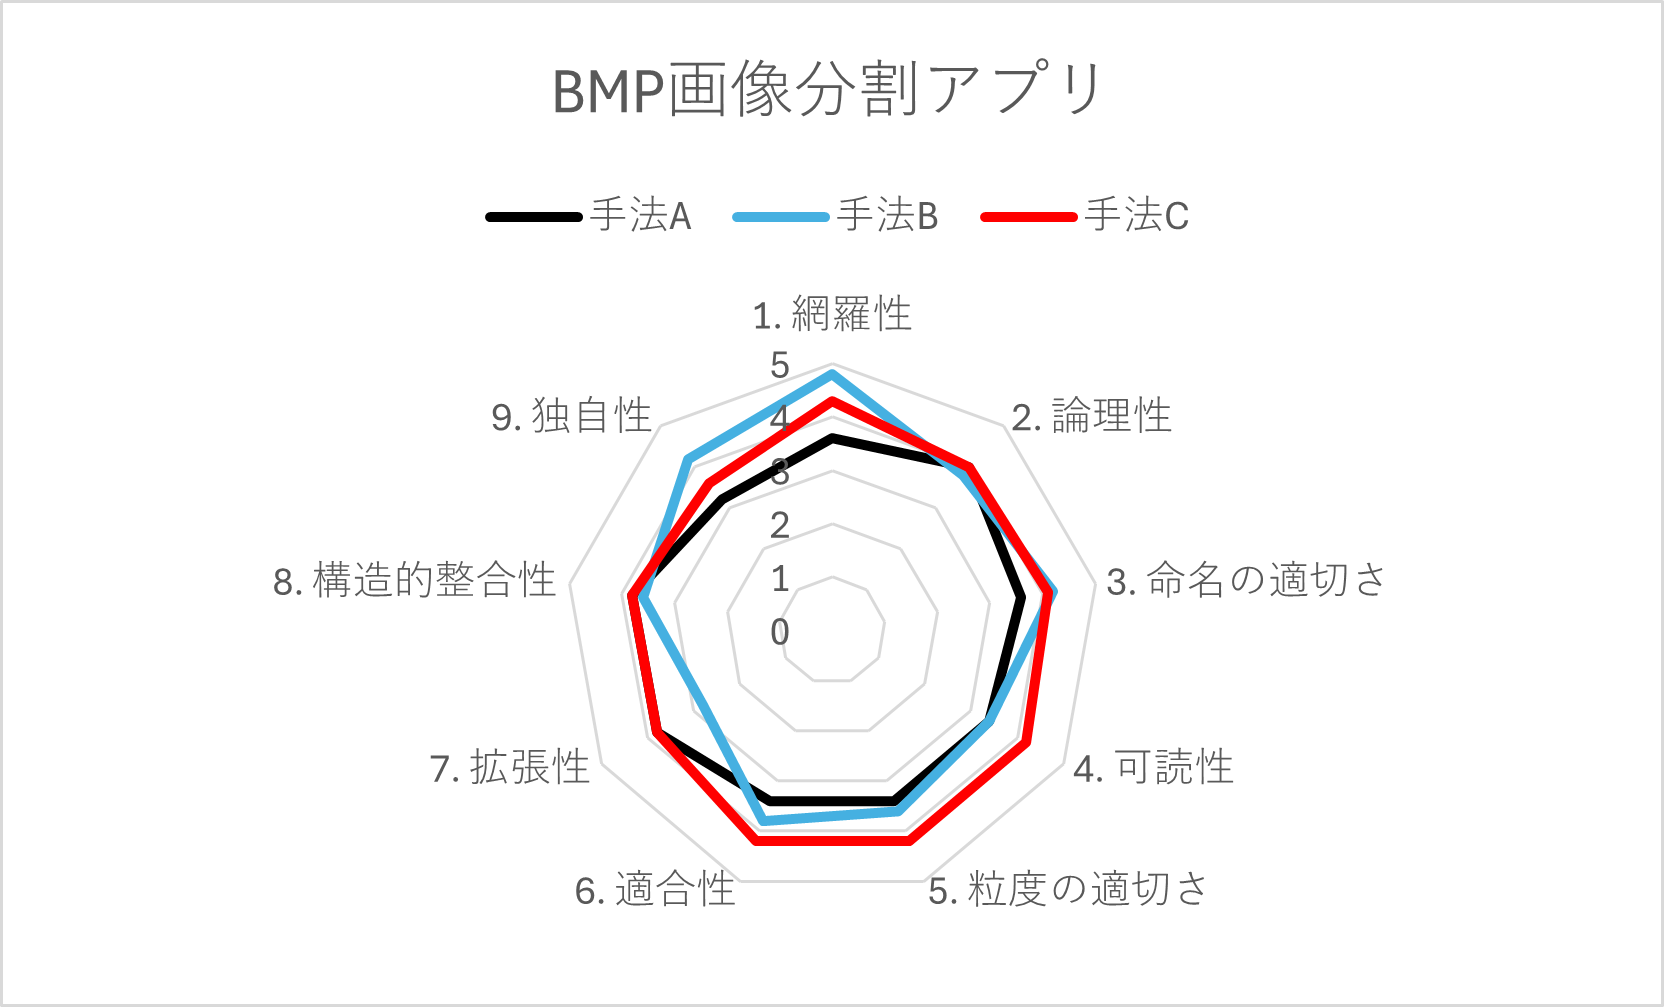
\includegraphics[width=0.8\textwidth]{images/BMPラベル.png}
  \caption{BMP画像分割アプリの評価結果のレーダーチャート}
  \label{fig:bmpchart}
\end{figure}

\begin{figure}[H]
  \centering
  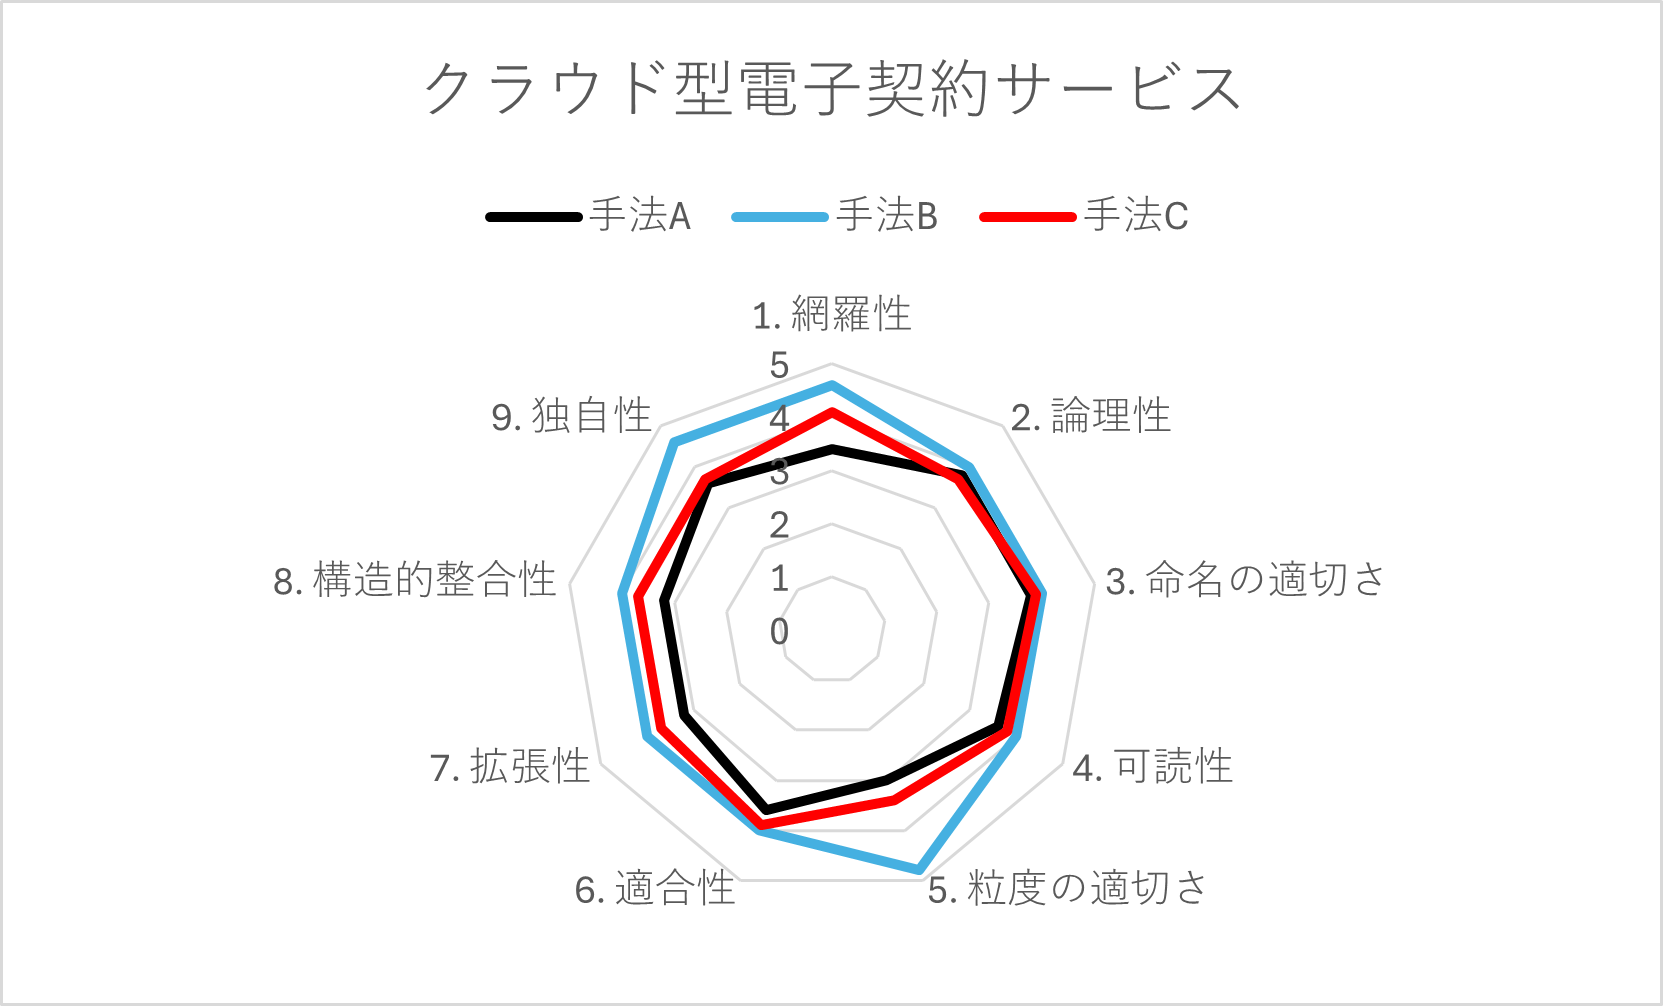
\includegraphics[width=0.8\textwidth]{images/クラウドラベル.png}
  \caption{クラウド型電子契約サービスの評価結果のレーダーチャート}
  \label{fig:cloudchart}
\end{figure}




% \begin{table}[H]
%   \caption{BMP画像分割アプリの評価結果}
%   \label{tb:bmp}
%   \centering
%   \begin{tabular}{|l|c|c|c|c|}
%     \hline
%     \textbf{評価項目} & \textbf{手法A} & \textbf{手法B} & \textbf{被験者Bによる手法C} & \textbf{被験者Dによる手法C} \\
%     \hline\hline
%     1. 網羅性 & 3.6 & 4.8 & 4.4 & 4.2  \\
%     \hline
%     2. 論理性 & 4 & 3.8 & 4.2 & 3.8 \\
%     \hline
%     3. 命名の適切さ & 3.6 & 4.2 & 4.2 & 4  \\
%     \hline
%     4. 可読性 & 3.4 & 3.4 & 4.4 & 4  \\
%     \hline
%     5. 粒度の適切さ & 3.4 & 3.6 & 4.2 & 4.2 \\
%     \hline
%     6. 適合性 & 3.4 & 3.8 & 4.4 & 4 \\
%     \hline
%     7. 拡張性 & 3.8 & 2.8 & 4 & 3.6 \\
%     \hline
%     8. 構造的整合性 & 3.8 & 3.6 & 3 & 4 \\
%     \hline
%     9. 独自性 & 3.2 & 4.2 & 3.6 & 3.6 \\
%     \hline
%   \end{tabular}
% \end{table}

% \begin{table}[H]
%   \caption{クラウド型電子契約サービスの評価結果}
%   \label{tb:cloud}
%   \centering
%   \begin{tabular}{|l|c|c|c|c|}
%     \hline
%     \textbf{評価項目} & \textbf{手法A} & \textbf{手法B} & \textbf{被験者Aによる手法C} & \textbf{被験者Cによる手法C} \\
%     \hline\hline
%     1. 網羅性 & 3.4 & 4.6 & 4 & 4.2  \\
%     \hline
%     2. 論理性 & 3.8 & 4 & 3.6 & 3.8  \\
%     \hline
%     3. 命名の適切さ & 3.8 & 4 & 4 & 3.8  \\
%     \hline
%     4. 可読性 & 3.6 & 4 & 3.8 & 3.8  \\
%     \hline
%     5. 粒度の適切さ & 3 & 4.8 & 2.8 & 4  \\
%     \hline
%     6. 適合性 & 3.6 & 4 & 3.8 & 4  \\
%     \hline
%     7. 拡張性 & 3.2 & 4 & 4 & 3.4 \\
%     \hline
%     8. 構造的整合性 & 3.6 & 4 & 3.8 & 3.6 \\
%     \hline
%     9. 独自性 & 2.8 & 4.6 & 3.8 & 3.6 \\
%     \hline
%   \end{tabular}
% \end{table}















% 本節では、5人の評価者による詳細な評価結果を示す。
% 表\ref{tb:detailed_evaluation_results_A}、表\ref{tb:detailed_evaluation_results_B}、表\ref{tb:detailed_evaluation_results_C}に、各手法で作成された章立てに対する評価者ごとの評価点と、各評価項目の平均値を示す。





% 上記の表より、手法C(提案するプロンプト)がすべての評価項目において最も高い平均スコアを記録していることが分かる。
% 特に「構造的整合性」では全評価者が5点を付けており、提案するプロンプトの有効性が明確に示されている。
% また、評価者間のばらつきも手法Cが最も小さく、安定した品質の章立てが生成されていることが確認できる。

% \section{実験結果}
% 本節では、2つの対象システムについて、各手法で作成した章立ての評価結果を示す。
% システムごとに評価結果の概要を示した後、作成した章立ての詳細と考察を述べる。

% \subsection{BMP画像分割アプリにおける章立ての評価結果}

% \subsubsection{評価結果の概要}
% BMP画像分割アプリについて、手法A(被験者A)、手法B(被験者C)、手法C(被験者BとD)が作成した章立ての評価結果を表\ref{tb:evaluation_result_bmp}に示す。

% \begin{table}[H]
%   \caption{BMP画像分割アプリの評価結果}
%   \label{tb:evaluation_result_bmp}
%   \centering
%   \begin{tabular}{|l|c|c|c|}
%     \hline
%     \textbf{評価項目} & \textbf{手法A} & \textbf{手法B} & \textbf{手法C(平均)} \\
%     \hline\hline
%     1. 網羅性 & 3.5 & 4.0 & \textbf{4.8} \\
%     \hline
%     2. 論理性 & 4.0 & 3.5 & \textbf{4.5} \\
%     \hline
%     3. 命名の適切さ & 3.8 & 3.5 & \textbf{4.2} \\
%     \hline
%     4. 可読性 & 3.2 & 3.8 & \textbf{4.6} \\
%     \hline
%     5. 粒度の適切さ & 3.0 & 2.5 & \textbf{4.0} \\
%     \hline
%     6. 適合性 & 3.5 & 3.5 & \textbf{4.7} \\
%     \hline
%     7. 拡張性 & 3.0 & 3.8 & \textbf{4.3} \\
%     \hline
%     8. 構造的整合性 & 3.8 & 3.2 & \textbf{4.9} \\
%     \hline
%     9. 独自性 & 3.0 & 3.0 & \textbf{4.0} \\
%     \hline
%   \end{tabular}
% \end{table}

% 表\ref{tb:evaluation_result_bmp}より、提案するプロンプトを用いた手法(手法C)がすべての評価項目において最も高いスコアを記録した。
% 特に「網羅性」(4.8)、「可読性」(4.6)、「適合性」(4.7)、「構造的整合性」(4.9)において顕著な高評価を得ており、提案するプロンプトの有効性が確認出来た。
% 手法Aは「論理性」(4.0)において比較的高いスコアを示したが、「粒度の適切さ」(3.0)や「拡張性」(3.0)では低い評価となった。
% 手法Bは全体的に中程度の評価であり、特に「粒度の適切さ」(2.5)と「構造的整合性」(3.2)において改善の余地が見られた。

% \clearpage
% % \begin{minipage}{\textwidth}
% \subsubsection{作成した章立ての詳細}
% 各手法で作成した章立ての詳細を以下に示す。

% \paragraph{手法A(手動作成)による章立て}
% 図\ref{fig:A_chapter_structure_of_bmp_app}に、手法Aで作成した章立てを示す。
% この章立ては、被験者がLLMを使用せず、自身の経験と知識に基づいて作成したものである。



% 全体として9章で構成され、比較的シンプルな構造となっている。
% 「概要」「基本条件」「構成」「機能」「運用」「セキュリティ」「安全設計」「データ仕様」「付帯事項」という基本的な項目は網羅されているが、階層構造が浅く、粒度の適切さに欠ける部分が見られる。
% 特に、第3章「構成」において節番号の付け方に不整合があり(3.1, 3.2ではなく1., 2.となっている)、構造的整合性の評価が低くなった要因と考えられる。
% また、第6章「セキュリティ」と第7章「安全設計」が節レベルの詳細を持たず、拡張性に課題がある。
% % \end{minipage}
% % \clearpage
% \begin{minipage}{\textwidth}
% \paragraph{手法B(自由プロンプト)による章立て}
% 図\ref{fig:B_chapter_structure_of_bmp_app}に、手法Bで作成した章立てを示す。
% この章立ては、被験者がLLMを使用したが、本研究のプロンプトは使用せず、自由な指示で作成したものである。


% \clearpage
% 全体として10章で構成し、手法Aと比較して詳細な階層構造を持つ。
% 「用語・略語定義」や「画像分割処理仕様」など、手法Aにはない独自の章が含んでおり、網羅性が向上している。
% また、各章が適切に節・項に分割されており、可読性が高い。
% しかし、第5章「画像分割処理仕様」が独立した章として存在する一方で、第4章「機能仕様」との関係が不明瞭であり、論理性の評価が低くなった。
% また、粒度の適切さについては、項レベルまで細分化されているものの、内容の粒度が不均一であり、改善の余地がある。

% \clearpage
% \begin{minipage}{\textwidth}
% \paragraph{手法C(提案するプロンプト)による章立て}
% 図\ref{fig:C_chapter_structure_of_bmp_app_1}と図\ref{fig:C_chapter_structure_of_bmp_app_2}に、手法Cを用いて作成した2つの章立てを示す。
% これらは、被験者BとDがそれぞれ本研究のテンプレートプロンプトを用いて作成したものである。




% 両者とも10〜11章で構成され、体系的かつ詳細な階層構造を持つ。
% 共通して「概要」「動作環境・前提条件」「システム全体像/仕様」「画面仕様」「機能仕様」「エラー仕様」「非機能要件」「データ仕様」「運用仕様」「テスト観点」という項目が含まれており、高い網羅性を示している。
% 特に、「ユースケース」「画面仕様」「非機能要件」「テスト観点整理」など、手法AやBにはない項目が含まれており、新人プログラマにとって理解しやすい構成となっている(適合性の高評価)。
% また、章・節・項の階層構造が一貫しており、構造的整合性が非常に高い。
% 2つの章立ての違いとしては、章の順序(「システム全体像」と「動作環境」の順番)や、「ユースケース」の独立性などが挙げられるが、いずれも論理的な構成となっている。

% \clearpage
% \begin{minipage}{\textwidth}
% \subsubsection{考察}
% BMP画像分割アプリの評価結果から、以下の知見が得られた。

% \begin{itemize}
%     \item \textbf{提案するプロンプトの優位性}: 提案するプロンプトを用いた手法(手法C)は、すべての評価項目において最も高いスコアを記録し、特に「網羅性」「適合性」「構造的整合性」において顕著な優位性を示した。これは、テンプレートプロンプトが「ベース章立て」と「出力指示」を明示的に提供することで、体系的かつ一貫性のある章立てを生成できることを示している。
    
%     \item \textbf{手動作成の課題}: 手法Aは、経験に基づいた論理的な構成を示したものの、粒度の適切さや拡張性において課題が見られた。特に、階層構造の不整合(第3章の節番号)は、手動作成における見落としの可能性を示唆している。
    
%     \item \textbf{自由プロンプトの使用の限界}: 手法Bは、手法Aよりも詳細な章立てを生成したが、章の論理的な関係性や粒度の均一性において改善の余地があった。これは、明確な指示がない場合、LLMが生成する章立ての品質にばらつきが生じることを示している。
    
%     \item \textbf{提案するプロンプトの再現性}: 手法Cで作成された2つの章立ては、異なる被験者によって作成されたにもかかわらず、高い類似性と一貫性を示した。これは、テンプレートプロンプトが再現性の高い章立て生成を可能にすることを示している。
% \end{itemize}
% \end{minipage}

% \subsection{クラウド型電子契約サービスにおける章立ての評価結果}

% \subsubsection{評価結果の概要}
% クラウド型電子契約サービスについて、手法A(被験者B)、手法B(被験者D)、手法C(被験者AとC)で作成された章立ての評価結果を表\ref{tb:evaluation_result_cloud}に示す。

% \begin{table}[H]
%   \caption{クラウド型電子契約サービスの評価結果}
%   \label{tb:evaluation_result_cloud}
%   \centering
%   \begin{tabular}{|l|c|c|c|}
%     \hline
%     \textbf{評価項目} & \textbf{手法A} & \textbf{手法B} & \textbf{手法C(提案するプロンプト)} \\
%     \hline\hline
%     1. 網羅性 & 3.5 & 3.5 & \textbf{4.8} \\
%     \hline
%     2. 論理性 & 4.0 & 2.5 & \textbf{4.5} \\
%     \hline
%     3. 命名の適切さ & 3.8 & 3.5 & \textbf{4.2} \\
%     \hline
%     4. 可読性 & 3.2 & 3.2 & \textbf{4.6} \\
%     \hline
%     5. 粒度の適切さ & 3.0 & 2.5 & \textbf{4.0} \\
%     \hline
%     6. 適合性 & 3.5 & 3.0 & \textbf{4.7} \\
%     \hline
%     7. 拡張性 & 3.0 & 3.2 & \textbf{4.3} \\
%     \hline
%     8. 構造的整合性 & 3.8 & 2.8 & \textbf{4.9} \\
%     \hline
%     9. 独自性 & 3.0 & 3.0 & \textbf{4.0} \\
%     \hline 
%   \end{tabular}
% \end{table}

% 表\ref{tb:evaluation_result_cloud}より、BMP画像分割アプリと同様に、提案するプロンプトを用いた手法(手法C)がすべての評価項目において最も高いスコアを記録した。
% 特に「網羅性」(4.8)、「可読性」(4.6)、「適合性」(4.7)、「構造的整合性」(4.9)において顕著な高評価を得ており、システムの複雑さに関わらず提案するプロンプトの有効性が確認された。
% 手法Aは「論理性」(4.0)において比較的高いスコアを示したが、BMP画像分割アプリと同様に「粒度の適切さ」(3.0)や「拡張性」(3.0)では低い評価となった。
% 手法Bは、特に「論理性」(2.5)と「構造的整合性」(2.8)において低い評価を受けており、複雑なシステムにおいて自由プロンプトでの章立て作成の難しさが示された。

% \clearpage
% \subsubsection{作成した章立ての詳細}
% 各手法で作成した章立ての詳細を以下に示す。

% % \begin{minipage}{\textwidth}
% \paragraph{手法A(手動作成)による章立て}
% 図\ref{fig:A_chapter_structure_of_cloud_contract_system}に、手法Aで作成した章立てを示す。


% 全体として9章で構成され、BMP画像分割アプリの手法Aと類似した構造を持つ。
% 「概要」「システム基本条件」「システム構成」「システムの機能」「システムの運用」「セキュリティ」「安全設計」「データ仕様」「付帯事項」という基本的な項目は網羅されているが、クラウドサービス特有の「画面仕様」や「外部インターフェース」などの項目が不足している。
% また、第4章「システムの機能」の項レベル(4.2.1〜4.2.4)において、番号の付け方に不整合があり(スペースがない)、構造的整合性に課題がある。
% 第2章「システム基本条件」の2.6「以降環境」は「移行環境」の誤記と思われ、命名の適切さにも問題が見られる。
% % \end{minipage}

% \clearpage
% \begin{minipage}{\textwidth}
% \paragraph{手法B(自由プロンプト)による章立て}
% 図\ref{fig:B_chapter_structure_of_cloud_contract_system}に、手法Bで作成した章立てを示す。


% \end{minipage}
% \clearpage
% 全体として11章で構成され、非常に詳細な章立てとなっている。
% 「画面仕様」「セキュリティ設計」「安全性・法的要件」「非機能要件」など、クラウド型電子契約サービスに必要な項目が網羅されており、手法Aと比較して高い網羅性を示している。
% 特に、第7章「セキュリティ設計」と第8章「安全性・法的要件」が独立して存在し、電子契約サービスの重要な要素が適切に扱われている。
% しかし、章の配置に論理的な問題が見られる。例えば、第2章「システム基本条件」の2.4「性能・可用性要件」と第10章「非機能要件」の10.1「性能要件」、10.2「可用性要件」が重複しており、情報の整理が不十分である。
% また、第4章「機能仕様」と第5章「画面仕様」の関係が不明瞭であり、論理性の評価が低くなった要因と考えられる。

% \clearpage
% \begin{minipage}{\textwidth}
% \paragraph{手法C(提案するプロンプト)による章立て}
% 図\ref{fig:C_chapter_structure_of_cloud_contract_system_1}と図\ref{fig:C_chapter_structure_of_cloud_contract_system_2}に、手法Cで作成された2つの章立てを示す。


% \end{minipage}


% \clearpage
% \begin{minipage}{\textwidth}
% \end{minipage}

% 両者とも13章で構成され、非常に体系的かつ詳細な階層構造を持つ。
% 共通して「概要」「システム全体像」「動作環境・基本条件」「画面仕様」「機能仕様」「操作フロー」「外部インターフェース/データ仕様」「エラー仕様」「セキュリティ/非機能要件」「運用仕様」「テスト観点」「付録」という項目が含まれており、クラウド型電子契約サービスに必要な要素が網羅されている。
% 特に、「ユースケース」「操作フロー仕様」「外部インターフェース仕様」「テスト観点整理」など、複雑なシステムの理解に必要な項目が適切に配置されており、高い適合性を示している。
% また、章・節・項の階層構造が一貫しており、構造的整合性が非常に高い。
% 2つの章立ての違いとしては、「画面仕様」と「機能仕様」の順序、「セキュリティ仕様」の独立性などが挙げられるが、いずれも論理的な構成となっている。

% \subsubsection{考察}
% クラウド型電子契約サービスの評価結果から、以下の知見が得られた。

% \begin{itemize}
%     \item \textbf{複雑なシステムにおける提案するプロンプトの有効性}: BMP画像分割アプリと同様に、提案するプロンプトを用いた手法(手法C)はすべての評価項目において最も高いスコアを記録した。特に、クラウド型電子契約サービスのような複雑なシステムにおいても、提案するプロンプトが高品質な章立てを生成できることを確認した。
    
%     \item \textbf{システム規模による影響}: クラウド型電子契約サービスは、BMP画像分割アプリと比較してシステム規模が大きく、必要な章立ての項目も多い。手法Bは、BMP画像分割アプリでは比較的良好な評価を得たが、クラウド型電子契約サービスでは論理性と構造的整合性において低い評価を受けた。これは、システムの複雑さが増すほど、明確な指示がない場合のLLMの章立て生成の品質が低下することを示唆している。
    
%     \item \textbf{ドメイン知識の重要性}: 手法Aは、BMP画像分割アプリと同様の構造を採用したが、クラウド型電子契約サービス特有の「画面仕様」や「外部インターフェース」などの項目が不足していた。これは、手動作成においてドメイン知識が重要であることを示している。一方、提案するプロンプトを用いた手法は、テンプレートプロンプトによってドメイン知識を補完し、高品質な章立てを生成できることを確認した。
    
%     \item \textbf{提案するプロンプトの柔軟性}: 手法Cを用いて作成した2つの章立ては、章の順序や項目の配置に若干の違いがあるものの、いずれも高い評価を得た。これは、テンプレートプロンプトが一定の柔軟性を持ちながらも、品質を保証できることを示している。
% \end{itemize}

% \subsection{実験結果の分析}

% \subsubsection{全体的な傾向}
% 2つのシステムにおける評価結果を総合的に比較した結果を、表\ref{tb:evaluation_result_summary}に示す。

% \begin{table}[H]
%   \caption{全体の評価結果の平均}
%   \label{tb:evaluation_result_summary}
%   \centering
%   \begin{tabular}{|l|c|c|c|}
%     \hline
%     \textbf{評価項目} & \textbf{手法A} & \textbf{手法B} & \textbf{手法C} \\
%     \hline\hline
%     1. 網羅性 & 3.5 & 3.8 & \textbf{4.8} \\
%     \hline
%     2. 論理性 & 4.0 & 3.0 & \textbf{4.5} \\
%     \hline
%     3. 命名の適切さ & 3.8 & 3.5 & \textbf{4.2} \\
%     \hline
%     4. 可読性 & 3.2 & 3.5 & \textbf{4.6} \\
%     \hline
%     5. 粒度の適切さ & 3.0 & 2.5 & \textbf{4.0} \\
%     \hline
%     6. 適合性 & 3.5 & 3.2 & \textbf{4.7} \\
%     \hline
%     7. 拡張性 & 3.0 & 3.5 & \textbf{4.3} \\
%     \hline
%     8. 構造的整合性 & 3.8 & 3.0 & \textbf{4.9} \\
%     \hline
%   \end{tabular}
% \end{table}

% 図\ref{fig:result_chart}に、各手法の評価結果をレーダーチャートで比較したものを示す。

% \begin{figure}[H]
%   \centering
%   % TODO: ここにExcel等で作成したレーダーチャートの画像を差し替える (images/result_chart.pdf)
%   \includegraphics[width=0.8\linewidth]{images/syokuji_computer.png} % 仮の画像
%   \caption{実験結果の比較(レーダーチャート)}
%   \label{fig:result_chart}
% \end{figure}

% \subsubsection{提案するプロンプトの有効性}
% 実験の結果、提案するプロンプトを用いた手法(手法C)は、すべての評価項目において手法Aおよび手法Bを上回るスコアを記録した。
% 特に「網羅性」(4.8)、「可読性」(4.6)、「適合性」(4.7)、「構造的整合性」(4.9)において顕著な高さを示しており、これはプロンプトで与えた「ベース章立て」と「出力指示」の有効性を示唆している。

% 提案するプロンプトの優位性は、以下の要因によるものと考えられる：

% \begin{enumerate}
%     \item \textbf{体系的な構造}: テンプレートプロンプトが提供する「ベース章立て」により、システム仕様書に必要な項目が網羅的に含まれる。
    
%     \item \textbf{一貫性の確保}: 「出力指示」により、章・節・項の階層構造が一貫して適用され、構造的整合性が高まる。
    
%     \item \textbf{ドメイン知識の補完}: テンプレートプロンプトが、システム仕様書作成に必要なドメイン知識を提供し、経験の浅い被験者でも高品質な章立てを作成できる。
    
%     \item \textbf{再現性の高さ}: 異なる被験者が同じテンプレートプロンプトを使用することで、類似した高品質な章立てが生成出来る。
% \end{enumerate}

% \subsubsection{手法間の比較}
% 手法A(手動作成)は、「論理性」において比較的高いスコアを示したが、「粒度の適切さ」や「拡張性」では低い評価となった。
% これは、経験に基づいた論理的な構成は可能であるものの、詳細な階層構造の設計や将来の拡張を考慮した設計には課題があることを示している。

% 手法B(自由プロンプト)は、全体的に中程度の評価であり、特に「粒度の適切さ」と「構造的整合性」において改善の余地が見られた。
% また、システムの複雑さが増すほど、論理性の評価が低下する傾向が見られた。
% これは、明確な指示がない場合、LLMが生成する章立ての品質にばらつきが生じることを示している。

